\documentclass[class=article,border=5pt]{standalone}

\usepackage[usenames,dvipsnames]{xcolor}

\usepackage{tikz}
\usetikzlibrary{arrows,shapes,fit,backgrounds,calc}

\usepackage{amsmath,amsfonts,amsthm,amssymb,mathtools}

\usepackage{../luke-macros}

\pgfdeclarelayer{background}
\pgfsetlayers{background,main}

\setlength{\parskip}{0pt}
\setlength{\parindent}{0pt}

\begin{document}

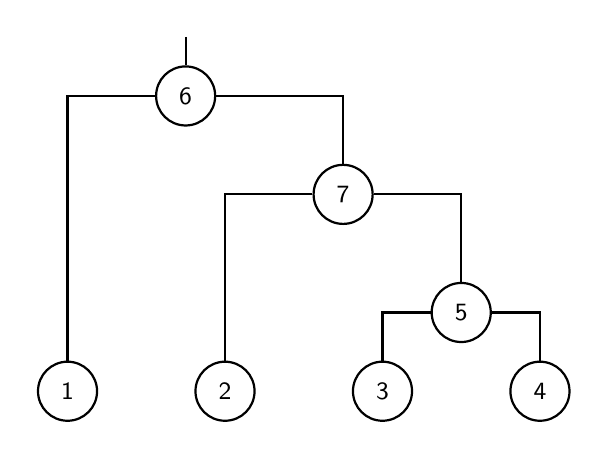
\begin{tikzpicture}
    \sffamily

    \tikzset{ST/.style={draw=black,solid,thick}}
    \tikzset{SN/.style={thick,circle,inner sep=0mm,minimum size=0.75cm,font=\small,draw}}
    \tikzset{HS/.style={thick,shape=rectangle,rounded corners}}

    \node (a) at (-1.5, 4.5) {};
    	\node (6) [SN] at (-1.5, 3.75) {6};
    		\node (1) [SN] at (-3, 0) {1};
    		\node (7) [SN] at (0.5, 2.5) {7};
                \node (2) [SN] at (-1, 0) {2};
    			\node (5) [SN] at (2, 1) {5};
    				\node (3) [SN] at (1, 0) {3};
    				\node (4) [SN] at (3, 0) {4};

    \begin{pgfonlayer}{background}
        \node[HS, fit = (1)(2)(3)(4)(5)(6)(7)] () {};
    	\path[ST] (a.center) -- (6);
    		\path[ST] (6) -| (1);
    		\path[ST] (6) -| (7);
                \path[ST] (7) -| (2);
    			\path[ST] (7) -| (5);
    				\path[ST] (5) -| (3);
    				\path[ST] (5) -| (4);
    \end{pgfonlayer}
\end{tikzpicture}

\end{document}
